\documentclass[tikz,margin=5mm]{standalone}
\usepackage{tikz}
\begin{document}
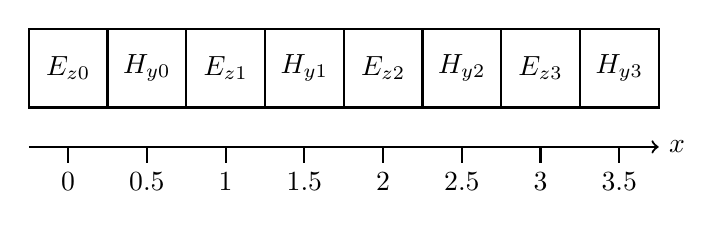
\begin{tikzpicture}[scale=1]

\foreach \i/\val in {
    0/$E_{z0}$,
    1/$H_{y0}$,
    2/$E_{z1}$,
    3/$H_{y1}$,
    4/$E_{z2}$,
    5/$H_{y2}$,
    6/$E_{z3}$,
    7/$H_{y3}$,
} {
    \draw[thick] (\i,0.25) rectangle ++(1,1);
    \node at (\i+0.5,0.75) {\val};
}

% draw an X axis below the chart
\draw[->, thick] (0,-0.25) -- (8,-0.25) node[right] {$x$};

\foreach \i in {0,...,7} {
    \draw[thick] (\i+0.5,-0.25) -- (\i+0.5,-0.45); % ticks
    \node[below] at (\i+0.5,-0.45) {\pgfmathparse{0.5*\i}\pgfmathprintnumber{\pgfmathresult}};
}

\end{tikzpicture}
\end{document}
